\documentclass[a0,landscape]{a0poster}

%\usepackage{pstricks,pst-grad}
\usepackage{multicol,ragged2e}
\usepackage{amsmath}
\usepackage{amsfonts}
\usepackage{amssymb}
\usepackage[amssymb,cdot]{SIunits}
\usepackage[absolute,overlay]{textpos}
\usepackage{graphicx,amssymb}
\usepackage{xcolor}
\usepackage[justification=centering]{caption}

%\textblockcolour{gray}


% Discourage hyphenatiosudo apt-get install texlive-fulln - doesn't look as good in posters.
\hyphenpenalty=5000
\tolerance=1000

% Definition of some variables and colors
\setlength{\parindent}{0.0cm}
\setlength{\parskip}{1.0cm}

\newdimen\headerwidth
\setlength{\headerwidth}{114.9cm}
\newdimen\onecolwidth
\setlength{\onecolwidth}{112.0cm}
\newdimen\twocolwidth
\setlength{\twocolwidth}{56.0cm}
\newdimen\threecolwidth
\setlength{\threecolwidth}{35cm}
\newdimen\headerheight
\setlength{\headerheight}{12cm}


\newcommand{\dospace}{\vspace*{0.9cm}}

\newenvironment{poster}{
  \begin{center}
  \begin{minipage}[c]{0.98\textwidth}
}{
  \end{minipage}
  \end{center}
}

\newenvironment{pcolumn}[1]{
  \begin{minipage}{#1\textwidth}
  \begin{center}
}{
  \end{center}
  \end{minipage}
}

\newenvironment{pcol}[1]{
  \begin{minipage}[t]{#1}
%  \begin{center}
}{
%  \end{center}
  \end{minipage}
}

%%%%%%%%%%%%%%%%%%%%%%%%%%%%%%%%%%%%%%%%%%%%%%%%%%%%
%%%               Background                     %%%
%%%%%%%%%%%%%%%%%%%%%%%%%%%%%%%%%%%%%%%%%%%%%%%%%%%%
\newcommand{\background}[3]{
  \newrgbcolor{cgradbegin}{#1}
  \newrgbcolor{cgradend}{#2}
  \psframe[fillstyle=gradient,gradend=cgradend,
  gradbegin=cgradbegin,gradmidpoint=#3](-10,10)(1.1\textwidth,-1.1\textheight)
}

%%%%%%%%%%%%%%%%%%%%%%%%%%%%%%%%%%%%%%%%%%%%%%%%%%%%
%%%                myfig                         %%%
%%%%%%%%%%%%%%%%%%%%%%%%%%%%%%%%%%%%%%%%%%%%%%%%%%%%
\newcommand{\myfig}[3][0]{
\begin{center}
  \vspace{0.7cm}
  \includegraphics[width=#3\hsize,angle=#1]{#2}
  \nobreak
\end{center}}

%%%%%%%%%%%%%%%%%%%%%%%%%%%%%%%%%%%%%%%%%%%%%%%%%%%%
%%%                mycaption                     %%%
%%%%%%%%%%%%%%%%%%%%%%%%%%%%%%%%%%%%%%%%%%%%%%%%%%%%
\setcounter{figure}{0}
\newcommand{\mycaption}[1]{
  \vspace{0.1cm}
  \begin{quote}
    {\small \textbf{Figure \arabic{figure}:} #1}
  \end{quote}
  \vspace{0.3cm}
  \stepcounter{figure}
}

\newcommand{\pbox}[4]{
%\psshadowbox[#3]{
\begin{minipage}[t][#2][t]{#1}
#4
\end{minipage}
}%}

% Set up a grid with a border (first two arguments) and the number of intervals specified
\TPGrid[25mm,0mm]{115}{80}

\begin{document}

\begin{textblock}{115}(0, 0)
\begin{pcol}{\headerwidth}
%\pbox{0.98\textwidth}{}{
%% University logo
\begin{minipage}[c][\headerheight][c]{0.1\textwidth}
  \begin{center}
    
\includegraphics[width=1.0\textwidth]{images/Kitware}
  \end{center}
\end{minipage}
%%% Title
\begin{minipage}[c][\headerheight][c]{0.755\textwidth}
  \begin{center}
    {\Huge \textbf{Web-based Analysis and Visualization of Large Climate and Geospatial Datasets}}\\[10mm]
    {\Large \underline{Aashish Chaudhary}, Elo Leung, Chris Harris, Charles Doutriaux, Thomas Maxwell, Berk Geveci, Dean Williams, and Jerry Potter}\\[6.5mm]
    {\large Website: \texttt{http://uvcdat.llnl.gov}\hspace*{1.5cm} Email: \texttt{aashish.chaudhary@kitware.com}}\\[6.5mm]
    {\large Scientific Computing, Kitware, Inc, 28 Corporate Drive, Clifton Park, NY 12065.}
  \end{center}
\end{minipage}
%% ClimatePipes logo
\begin{minipage}[c][\headerheight][c]{0.1\textwidth}
  \begin{center}
    
\includegraphics[width=1.5\textwidth]{images/UV-CDAT_logo}
  \end{center}
\end{minipage}
%}
\end{pcol}
\end{textblock}

\dospace

%% Left column

%% INTRODUCTION
\begin{textblock}{35}(0, 13)
\begin{pcol}{\threecolwidth}

 \begin{center}\textbf{\begin{Large}Motivation\end{Large}}\end{center}

\large
At present, the majority of the climate science community still relies heavily on primitive analysis and visualization tools that are based on the thick (or fat) client application concept. This means that the user must download software to the appropriate machines or hardware where the data resides (e.g., laptops, desktops, or HPC machines). In such cases, the user encounters multiple levels of installation challenges such as finding the right prerequisite software packages, software versions, and currently supported hardware and operating systems.

Analysis and visualization tools have thus begun moving toward the thin client application concept, where the user installs very little software. In most cases, only a web browser is needed. In such cases, an analysis and visualization software is deployed on a central server rather than on each individual system, which eliminates the user’s installation and operating system requirement challenges. This approach also provides the flexibility to install the software on the user’s system using VM (virtual operating system) in case scientists need an installation.

Thin clients are well suited for environments in which the same information is going to be accessed by a general group of users. The tradeoff, however, is that thick clients provide users with more features, analysis and visualization, and interaction choices that make the software more customizable. Nevertheless, this trend is changing due to new web standards (HTML5) and more capable browsers that have been developed by leading web technology companies.

\vspace{1cm}
 \begin{center}\textbf{\begin{Large}Proposed Solution\end{Large}}\end{center}
\large
The need for highly scalable, collaborative, and easy to install and use software for large climate and geospatial data analysis and visualization led us to develop the CDATWeb toolkit. CDATWeb utilizes the latest in web-technologies such as RESTful API and HTML5 to provide powerful visualization and analysis capabilities on modern web-browsers. Underneath, it is built on top of UV-CDAT, ParaViewWeb, and DJango python web-framework. A complete architecture of CDATWeb is shown in Figure 1. The CDATWeb backend python API is developed on top of UV-CDAT to utilize its analysis and visualization capabilities. The web API of CDATWeb utilizes ParaViewWeb at its core. ParaViewWeb enables communication with a ParaView / UV-CDAT server running on a remote visualization node or cluster using a light-weight JavaScript API. By utilizing UV-CDAT and ParaViewWeb, CDATWeb provides capabilities including interactive 2D and 3D visualization, remote job submission and processing, and exploratory and batch-mode analysis for scientific models and observational datasets.

\vspace{1cm}
\begin{center}\textbf{\begin{large}JavaScript API and Thin Client\end{large}}\end{center}
\large

Our web-based analysis and visualization toolkit clients that use CDATWeb are considered smart clients. That is, they are based more on the traditional client-server architecture concept within the web-based model, as is shown in Figure 1. They are more similar to thick clients in that CDATWeb smart clients are Internet-connected devices that allow a user’s local applications to interact with server-based applications through the use of web services. As is the case with thick clients, this provides for increased analysis and visualization interaction, as well as software customization.

\end{pcol}
\end{textblock}

%% Central column

\begin{textblock}{35}(38.9, 13)
\begin{pcol}{\threecolwidth}

With CDATWeb, a user will be able to work offline via the locally installed CDATWeb backend (using VM) and access the appropriate local data or connect to the Internet and access distributed data from Earth System Grid Federation (ESGF). With this architecture in place, CDATWeb has the ability to be deployed and updated in real-time over the network from a centralized server, support multiple platforms and operating systems, and run on almost any device including mobile phones, notebooks, tablet PCs, laptops, desktops, and HPC machines.

The main goal of this design is to facilitate collaboration among distributed users by connecting them through a user-friendly, web-based system to conduct visualization and analysis on both real-time simulation and archived data sets with intuitive visual output and online steering capability. Figure 2 depicts how users access the CDATWeb client interface. It should be noted that the interface can be changed as per the requirement and need of a particular organization or project, as long as it uses the CDATWeb javascript API.

\begin{figure}[overview]
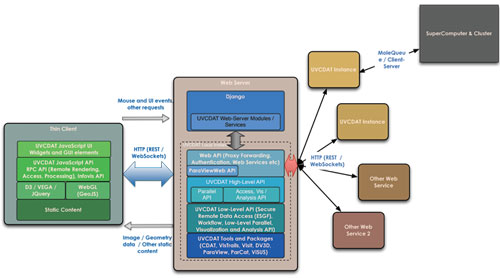
\includegraphics[height=0.6\hsize]{images/Overview}
\caption{Overview of the CDATWeb architecture}
\end{figure}

\vspace{1cm}
\begin{center}\textbf{\begin{large}Server Side Analysis and Visualization\end{large}}\end{center}

One of the important components of CDATWeb is server-side analysis and visualization. In this architecture, a web-server receives a request for data processing, analysis, or remote rendering from a thin client such as a web browser. A prerequisite to this is user authentication, which involves the user providing a username/password to the server. If the prerequisite is satisfied, upon receiving the request, the server may create a process specific to the user’s session (per session ID). A separate process per session strengthens security and offers solutions for scalability. Any subsequent requests for data processing are then forwarded to this process until the session ends. At this time, the process is deleted on the server side. Certain requests that do not require intensive computing are served directly by the web-server. For instance, accessing pre-computed climatology for diagnostics is served directly by the server. The server delivers most of the static content to thin clients, as needed.

In the design of server-side analysis, we have adopted standard protocols and communication channels between the client and the server. Most of the static content and some dynamic content for exploratory analysis are served in a RESTful manner. The client can access this content by invoking an AJAX call over the web. For interactive visualization and analysis, data is accessed via WebSockets, as it provides the required flexibility and interactivity.

The CDATWeb server-side analysis is built on top of an open-source parallel remote data processing framework known as ParaViewWeb. ParaViewWeb enables communication with a ParaView server running on a remote visualization node or cluster using a lightweight JavaScript API. Using this API, web applications can easily embed interactive 2D and 3D visualization components. Application developers can write simple

%% Right column
\begin{textblock}{35}(77.8, 13)
\begin{pcol}{35cm}

Python scripts to extend the server capabilities, including to create custom visualization pipelines. Essentially, we have utilized this ability to extend ParaViewWeb to support the remote rendering of VCS
and DV3D plots, as shown in Figure 3.  In the CDATWeb architecture, a plot on the frontend has its corresponding instance on the backend. Based on the plot type requested by the frontend, CDATWeb plot factory creates the corresponding plot type on the backend with a specific ID for that plot. Any subsequent calls to the newly created plot are then mapped via its ID by the backend.

We chose Python as the binding language for the server-side analysis. Python was the natural choice for the framework due to its support in the scientific computing community and widespread use in almost every field of computer science. In addition, a Python-based platform enabled us to integrate existing UV-CDAT source code on the backend with minimal effort.

\begin{figure}[montage]
  \vspace{0.7cm}
  \myfig[0]{images/vcs_plots}{0.80}
  \caption{CDATWeb client interface showing comparison between model output and observation}
\end{figure}


\begin{center}\textbf{\begin{large}Conclusion and Future Work\end{large}}\end{center}
We have presented some of our initial work in creating an open-source, web-based toolkit for the analysis and visualization of large climate datasets as part of the UV-CDAT project.  Although we did not describe the integration of CDATWeb with the diagnostics framework, it has been successfully demonstrated and deployed on a working system. The preliminary results are encouraging, as they have proven the usability of the toolkit in terms of its ease of use and effectiveness in providing a sophisticated computing and visualization environment for climate scientists.  We are very thankful to the Department of Energy (DOE) and NASA for providing the support required for this effort.

\begin{figure}[floodmap]
\myfig[1]{images/dv3d_plots}{0.80}
\caption{Remotely rendered VCS and DV3D plot in CDATWeb}
\end{figure}

\end{pcol}
\end{textblock}

\large
\end{pcol}
\end{textblock}

\begin{textblock}{115}(0, 73)

\includegraphics[height=0.04\hsize]{images/doe-logo}
\hspace{0.3cm}

\includegraphics[height=0.04\hsize]{images/VTK_logo}
\hspace{0.3cm}

\includegraphics[height=0.04\hsize]{images/UV-CDAT_logo}
\hspace{0.3cm}

\includegraphics[height=0.04\hsize]{images/esgf_1}
\hspace{0.3cm}

\includegraphics[height=0.04\hsize]{images/LLNL-Logo}
\hspace{0.3cm}

\includegraphics[height=0.04\hsize]{images/nasa}
\hspace{0.3cm}
\end{textblock}
\end{document}
